\section{EXPERIMENT}
In this section, we first describe the testbed and then present the results of the experiments.

\subsection{Testbed}

\subsubsection{Flapping Drone}

\begin{figure}
    \centering
    \begin{tabular}{cc}
        \begin{minipage}[h]{0.4 \columnwidth}
          \centering
          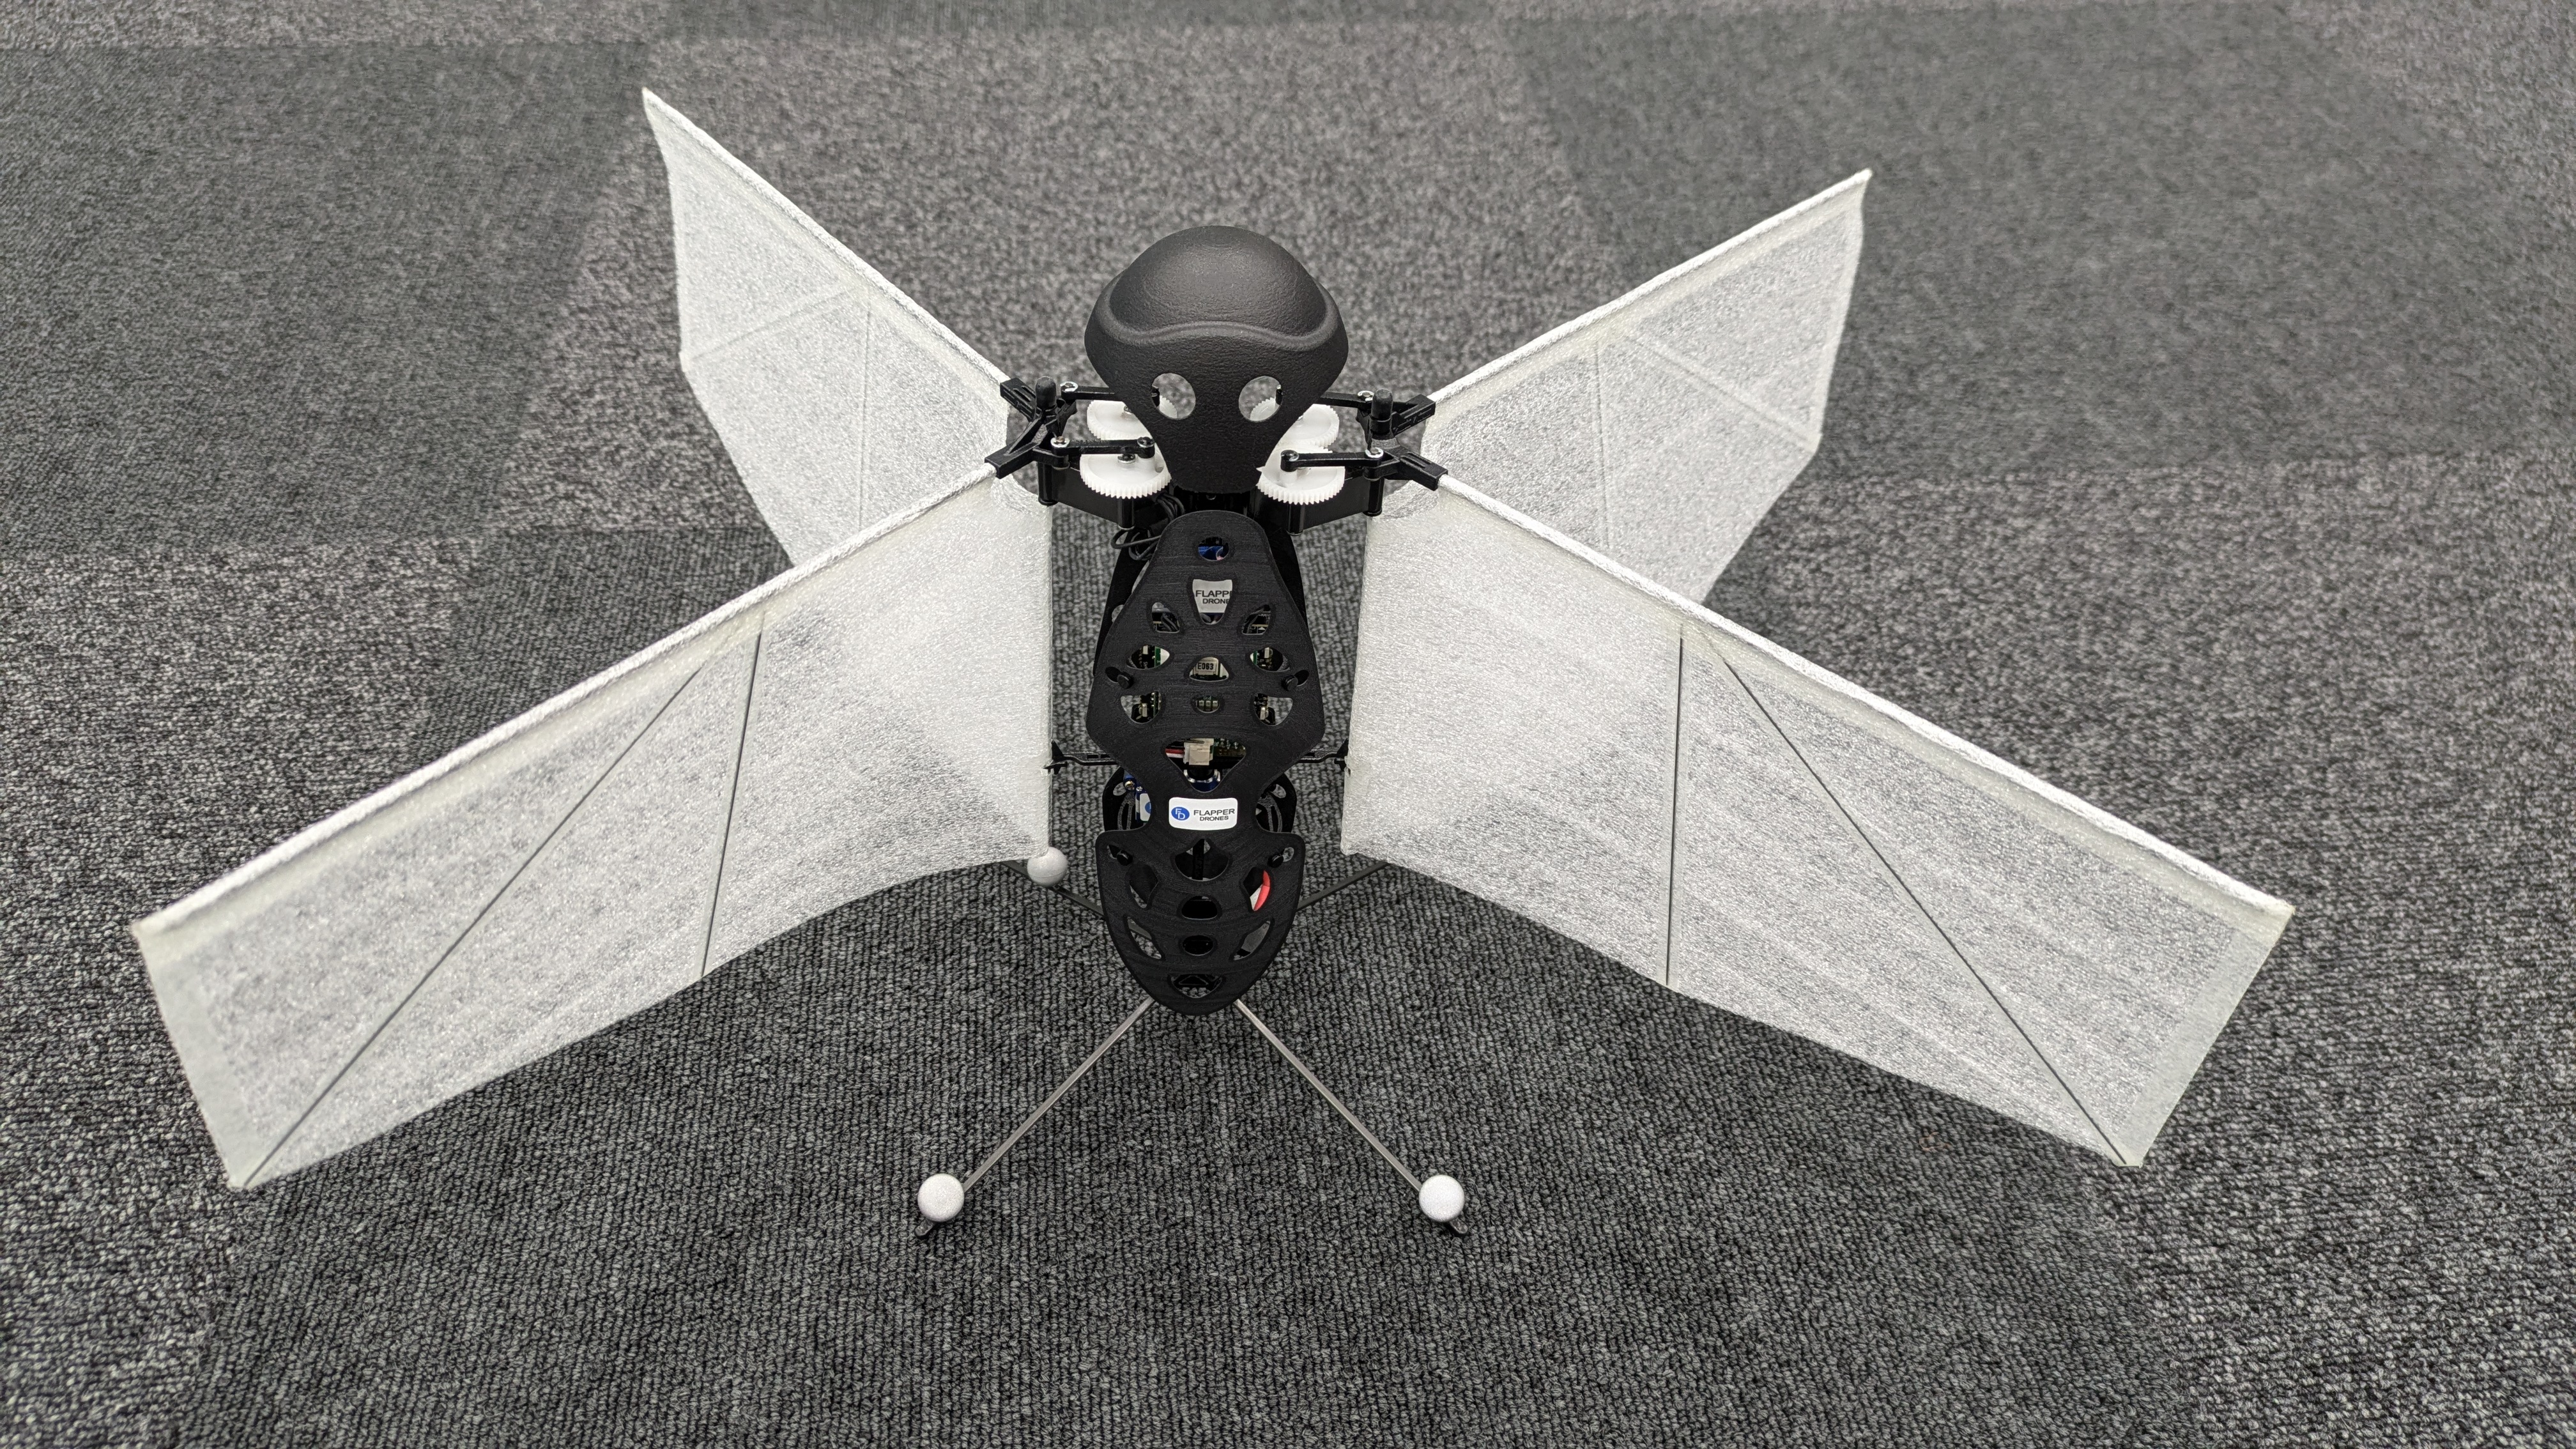
\includegraphics[keepaspectratio, scale=0.025]{flapper.jpg}
          \subcaption{}
          \label{fig:flapper}
        \end{minipage} &
        \begin{minipage}[h]{0.4 \columnwidth}
          \centering
          \includegraphics[keepaspectratio, scale=0.025]{leg.jpg}
          \subcaption{}
          \label{fig:leg}
        \end{minipage}
      \end{tabular}
    \caption{Flapper Nimble+ drone (a) and its leg with motion capture markers (b).}
\end{figure}

Flapper Nimble+ used in the experiment, shown in (\ref{fig:flapper}), is a bioinspired flapping-wing drone by FLAPPER DRONES compatible with the Crazyflie software, 
which is a open-source platform for research and development of quadcopters produced by Bitcraze AB. 
As shown in \ref{fig:leg} attached four motion capture markers on its legs for tracking its position and orientation. 

\subsubsection{Interface For Control}

\begin{figure}
  \centering
  \begin{tabular}{cc}
      \begin{minipage}[h]{0.4 \columnwidth}
        \centering
        \includegraphics[keepaspectratio, scale=0.025]{chest.jpg}
        \subcaption{}
        \label{fig:chest}
      \end{minipage} &
      \begin{minipage}[h]{0.4 \columnwidth}
        \centering
        \includegraphics[keepaspectratio, scale=0.025]{hand.jpg}
        \subcaption{}
        \label{fig:hand}
      \end{minipage}\\
      \begin{minipage}[h]{0.4 \columnwidth}
        \centering
        \includegraphics[keepaspectratio, scale=0.025]{chest_attach.jpg}
        \subcaption{}
        \label{fig:chest_attach}
      \end{minipage} &
      \begin{minipage}[h]{0.4 \columnwidth}
        \centering
        \includegraphics[keepaspectratio, scale=0.025, angle=90]{hand_attach.jpg}
        \subcaption{}
        \label{fig:hand_attach}
      \end{minipage}
    \end{tabular}
  \caption{Chest-mounted device (a) and wrist-mounted device (b) for controlling the state of flapping drone. The devices are attached to the user's body as illustrated in (c, d).}
\end{figure}

As noted in \ref{sec:motion-planning}-\ref{fig:trajectory}, the drone has to change its behavior according to the position of the user's palm.
To facilitate intuitive control, we designed a wearable interface consisting of:
\begin{itemize}
    \item A chest-mounted device shown in (\ref{fig:chest})
    \item A wrist-mounted device shown in (\ref{fig:hand})
\end{itemize}

Both devices were fabricated using a Bambu Lab X1-Carbon 3D printer. 
With these devices, we acquire the user's palm position and orientation from the motion capture system and calculate the desired drone behavior based on the user's palm position. 
This interaction design only requires arm bending and streaching to switch the state of the drone and thus enables a seamless and intuitive approach control.


\subsubsection{Experimental Environment}
The experiment was conducted in an enclosed indoor environment with the following specifications:
\begin{itemize}
    \item Room dimensions: [specify dimensions]
    \item Motion capture system: [specify system name]
\end{itemize}

A motion capture (MoCap) system was employed to track the positions of the hand, chest, and drone. Using these tracked positions, we developed an intuitive drone control interface that allows for natural interaction.


\subsection{Results and Analysis}

\subsubsection{Trajectory Mapping}
We mapped the actual flight trajectories of the drone in both 2D and 3D and compared them with the planned trajectory proposed in Section 3.

\subsubsection{Velocity Profile}
We analyzed the velocity profile of the drone to examine:
\begin{itemize}
    \item The presence or absence of overshoot.
    \item Whether the approach was perpendicular to the user’s palm.
\end{itemize}

\subsubsection{Success Rate Analysis}
The success rate of the system was evaluated by measuring the number of successful trials over multiple attempts. This metric was used to assess the reproducibility and reliability of the system.

\subsubsection{Distance Between Chest and Drone}
A distance-time graph was generated to verify whether the drone maintained a safe distance from the user during the experiment.

